\chapter{Project Vision}
\label{ch:vision}

This chapter describes what KhetLens is for. We first give an overview of the problem domain and a description of the system, then state the problem and break it into its parts. We then list our goals and objectives, define the scope, identify the Sustainable Development Goals the project supports, and record the constraints, the business opportunity and the stakeholders.

\section{Problem Domain Overview}
\label{sec:domain}
KhetLens sits where three areas meet: smallholder farming in Punjab, image-based plant pathology, and machine learning on low-cost phones.

Wheat is Pakistan's largest crop by area, with maize and cotton following among the field crops~\cite{fao_pakistan}; maize is grown in two seasons and supplies the poultry and livestock sector, and cotton is the main fibre crop of southern Punjab and the base of the textile industry. All three are grown mostly on small holdings. When a disease appears, the farmer relies on experience, neighbours, the local dealer, and occasional visits from extension staff. Timely, reliable diagnosis is the exception rather than the rule.

Many of the most damaging diseases of these crops show clearly on a leaf: the yellow stripes of wheat stripe rust, the scattered brown pustules of leaf rust, the long grey-brown lesions of maize northern leaf blight, the upward curling and thickened veins of cotton leaf curl. These are the symptoms a farmer notices and a phone camera can capture, whether in a close-up of one leaf or in a photograph of the plant taken from a short distance. A few conditions look alike in a photograph, for instance early rust and heat scorch, or bacterial blight and fungal leaf spot in cotton. Agronomists tell them apart using context, and the recent weather is one of the most useful clues, because fungal and viral epidemics are closely tied to temperature and humidity~\cite{ali2023striperust,ahmad2018clcuv}.

The phones farmers carry are entry-level Android devices with a few gigabytes of memory and no reliable connectivity. Modern mobile network architectures and model compression techniques~\cite{howard2019mnv3,hinton2015kd} make it practical to run a disease classifier on such a phone, provided the model is small, quantised and bundled with everything it needs.

\textbf{What the system does.} A farmer opens KhetLens, which has already fetched and stored the recent weather of their district the last time the phone was online. They photograph the affected plant, close up or from a short distance so that several leaves are visible. On the phone, the photo is checked for blur and poor lighting, analysed as a whole and in regions by a compact neural network that identifies the crop and the disease, scored for how confident and how familiar the result is, and adjusted using the recent weather. If the result is confident, the farmer sees the disease name in their language with an audio explanation and the reasons for the decision, and can open treatment and prevention guidance. If two conditions are close, the app asks up to three simple picture questions. If the photo is poor or shows something the model does not know, the app says so and suggests taking more photos rather than guessing. Each diagnosis is kept in the history for six months, and the farmer can report whether the diagnosis and treatment worked; that feedback is sent when the phone next has a connection and then removed from the phone. A library of all supported diseases, with audio, is available offline.

\section{Problem Statement}
Smallholder farmers in Punjab do not have quick, trustworthy access to leaf disease diagnosis for wheat, maize and cotton. Existing tools generally need an internet connection, are built and tested on laboratory-style images rather than field photographs, always give an answer even when the input is unclear, and present advice in languages and from sources that do not fit the local farmer. An offline, Urdu- and Punjabi-speaking application that diagnoses these three crops on an ordinary phone, uses local context to resolve look-alike symptoms, admits uncertainty, and gives locally reviewed treatment guidance is what we set out to build; we have not found an existing application that does this.

\section{Problem Elaboration}
We see the problem as four connected sub-problems.

\subsection{Working on real field photographs}
Published classifiers reach very high accuracy on curated datasets but lose a large part of it on photographs taken in fields, where the background, lighting, distance and framing vary and symptoms appear at different stages~\cite{mohanty2016,singh2020plantdoc}. Part of the cause is that models learn from the background and the photographic style as much as from the leaf~\cite{noyan2022bias}. Our model therefore has to be trained on field photographs from several regions, taken at a range of distances, augmented to reduce background shortcuts, tested only on field photographs, and complemented by photographs we collect locally.

\subsection{Telling apart conditions that look alike}
\label{sec:pairs}
Some pairs of conditions cannot be reliably separated from a single leaf image. For evaluation we designate three such pairs: rust against abiotic heat stress in wheat and maize; bacterial blight against fungal leaf spot in cotton; and leaf reddening against leaf curl virus in cotton. The recent weather is a cheap and available signal: stripe rust in Punjab, for example, develops within a specific range of temperature and humidity~\cite{ali2023striperust}, while heat scorch follows hot, dry spells. We need a way to use this signal that does not require a large paired dataset of images and weather.

\subsection{Knowing when not to answer}
A diagnosis tool that always answers can send a farmer to buy the wrong spray. The app has to recognise three different situations: a photograph too blurred or dark to use; a crop or object it was not trained on; and a disease of a supported crop that it has not seen. Each needs a different check and a different response (retake, decline, or ask questions), and all of them have to run on the phone. Plain softmax confidence is known to be over-confident~\cite{guo2017calibration}, so better-founded measures are needed.

\subsection{Reaching the farmer}
The application must work with no connection, on an entry-level phone, for a user who may read little and prefers Punjabi or Urdu. This means on-device inference, an icon-first interface, audio on every screen, locally reviewed treatment content, and an interface that explains its answers so that farmers come to trust it. Studies of agricultural advisory apps find that trust and visible results are what drive farmers' intention to adopt a tool~\cite{soodan2024adoption}.

\section{Goals and Objectives}
\label{sec:goals}
Our goal is to give wheat, maize and cotton farmers in Punjab a trustworthy, offline disease diagnosis tool in their own language. The objectives are:
\begin{enumerate}[label=\textbf{O\arabic*},leftmargin=2.2em]
  \item Diagnose the common leaf diseases of wheat, maize and cotton from a photograph of the plant, close up or from a short distance, with the model running on the phone.
  \item Run on entry-level Android phones, with a diagnosis returned within a couple of seconds and all farmer-facing features working offline.
  \item Use recent local weather to improve the separation of visually similar conditions.
  \item Recognise unusable photographs, unsupported crops and unfamiliar diseases, and respond with a retake request, follow-up questions or an honest ``not sure'' rather than a guess.
  \item Determine, through a structured study, how many locally collected field photographs are needed on top of public datasets.
  \item Present diagnoses, questions and guidance in English, Urdu and Punjabi with audio.
  \item Provide an offline disease library and an automatic short-term history of diagnoses.
  \item Base treatment guidance on Pakistani advisories and agricultural research, reviewed with our partner's agronomists.
  \item Collect farmer feedback on diagnosis and treatment outcomes to improve the system over time.
\end{enumerate}
We will measure O1 to O5 on a held-out set of field photographs and on the target class of phone, using accuracy and macro-F1, inference time and model size, calibration error and the false-positive rate of the uncertainty check; O6 to O9 will be verified through content review, test cases and feedback from farmers and field staff.

\section{Project Scope}
\label{sec:scope}
KhetLens covers three crops, wheat, maize and cotton, chosen for their area in Punjab and their importance to farmers. Within them it covers the conditions in Table~\ref{tab:classes}, selected because they are common in the region, visible on a leaf, and covered by available training data. The list will be confirmed with our partner's agronomists; fall armyworm damage in maize is a possible addition.

\begin{table}[H]
\centering\small
\caption{Conditions covered by KhetLens (17 classes).}
\label{tab:classes}
\begin{tabularx}{\textwidth}{|L{1.8cm}|Y|}
\hline
\textbf{Crop} & \textbf{Conditions} \\ \hline
Wheat (6) & Yellow (stripe) rust; brown (leaf) rust; powdery mildew; leaf blight / spot blotch; abiotic stress (heat scorch, nutrient deficiency); healthy \\ \hline
Maize (5) & Northern leaf blight; common rust; grey leaf spot; abiotic stress; healthy \\ \hline
Cotton (6) & Cotton leaf curl virus; bacterial blight; fungal leaf spot (Alternaria, target spot); leaf reddening; sucking-pest damage (whitefly, jassid); healthy \\ \hline
\end{tabularx}
\end{table}

\subsection{In scope}
\begin{itemize}
  \item Core diagnosis: on-device identification of crop and condition from a photograph of the plant, close up or from a short distance, fully offline.
  \item Context-aware diagnosis: adjustment of the image result using the recent weather of the farmer's district.
  \item Uncertainty handling: blur and exposure check, detection of unsupported or unfamiliar inputs, up to three picture-based follow-up questions, and an explicit ``not sure'' outcome.
  \item A three-language interface (English, Urdu, Punjabi) with recorded audio for all content.
  \item An offline disease library covering every supported condition.
  \item An automatic diagnosis history, kept for six months and then cleared.
  \item Treatment and prevention guidance drawn from Pakistani advisories and research, reviewed with agronomists, with the source shown.
  \item A farmer feedback mechanism that works offline and syncs when connected.
  \item Phone-number sign-in with a one-time code sent over WhatsApp, and a guest mode so that diagnosis never requires an account.
  \item Model and content updates downloaded when connected, without reinstalling the app.
  \item A small backend for verification, feedback collection and distribution of updates.
  \item A field-data efficiency study, carried out as part of model building rather than as a farmer-facing feature.
\end{itemize}

\subsection{Out of scope}
\begin{itemize}
  \item Crops other than wheat, maize and cotton, and diseases that show on stems, spikes, bolls or roots rather than leaves.
  \item Severity grading and detection of more than one disease on the same leaf.
  \item Voice input; audio is output only.
  \item Identifying pests from photographs of the insect itself.
  \item Prescriptive dosing; guidance names approved product types and refers to the label and the agronomist.
  \item A web dashboard for agronomists; we maintain the content ourselves and the agronomists review it offline.
  \item iOS and languages other than the three named.
\end{itemize}

\subsection{Deliverables}
The project will deliver the KhetLens Android application, the trained and compressed model, the content pack with audio, the backend service, the assembled datasets and the results of the field-data study, the project reports and a user manual.

\section{Sustainable Development Goal (SDG)}
KhetLens contributes primarily to \textbf{SDG 2, Zero Hunger}, and in particular to its target of raising the productivity and incomes of small-scale food producers. Earlier and more accurate diagnosis reduces losses on the three crops that matter most to Punjab's farmers, and it does so for the smallholder who can least afford the loss. The project also supports \textbf{SDG 12, Responsible Consumption and Production}, because guidance limited to approved products and label doses, and withheld when the diagnosis is uncertain, encourages more careful use of pesticides. Figure~\ref{fig:sdg} shows the full set of goals.

\begin{figure}[H]
    \centering
    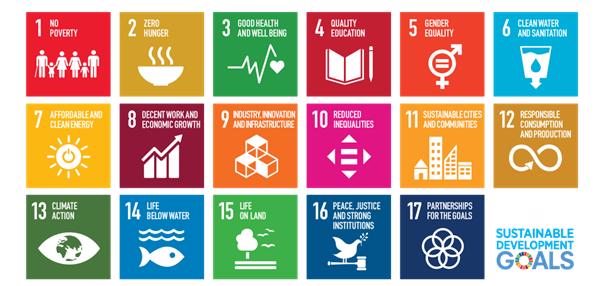
\includegraphics[width=0.7\textwidth]{Figures/Picture1}
    \caption[The seventeen UN Sustainable Development Goals; KhetLens targets Goals 2 and 12.]{The seventeen United Nations Sustainable Development Goals, shown as a grid of coloured tiles each with a number, a short title and an icon: 1 No Poverty, 2 Zero Hunger, 3 Good Health and Well-being, 4 Quality Education, 5 Gender Equality, 6 Clean Water and Sanitation, 7 Affordable and Clean Energy, 8 Decent Work and Economic Growth, 9 Industry, Innovation and Infrastructure, 10 Reduced Inequalities, 11 Sustainable Cities and Communities, 12 Responsible Consumption and Production, 13 Climate Action, 14 Life Below Water, 15 Life on Land, 16 Peace, Justice and Strong Institutions, 17 Partnerships for the Goals. KhetLens targets Goal 2 primarily and Goal 12 secondarily.}
    \label{fig:sdg}
\end{figure}

\section{Constraints}
\label{sec:constraints}
\begin{itemize}
  \item \textbf{Target hardware.} The app must run on entry-level Android phones with about 3\,GB of RAM and Android 8.1 or later, using the CPU only.
  \item \textbf{Connectivity.} All farmer-facing functions must work without a network; the network is used only when available and never blocks the farmer.
  \item \textbf{Storage.} The model, content and audio must fit comfortably on a low-cost phone; we are targeting a model under 10\,MB and a total install under 150\,MB.
  \item \textbf{Data.} Field photographs from Punjab depend on seasonal field visits with our partner; public datasets from other regions are used alongside them.
  \item \textbf{Language resources.} We record the Urdu and Punjabi audio ourselves so that terminology and pronunciation can be checked by the agronomists.
  \item \textbf{Content.} Treatment guidance must be consistent with Pakistan's pesticide regulations and provincial advisories and reviewed by an agronomist before release.
  \item \textbf{Privacy.} Photographs and precise location stay on the phone unless the farmer chooses to share them; only the district is stored on the server.
  \item \textbf{Academic.} Two semesters, three students, and limited GPU time through Colab, Kaggle and the university's GPU server.
\end{itemize}

\section{Business Opportunity}
Our immediate route to farmers is our industry partner. Fatima Fertiliser has a nationwide network of dealers and field officers through which KhetLens can be demonstrated and supported, and its agronomists give the treatment content a credibility that a student application could not establish alone. For the partner, an offline diagnosis tool strengthens its relationship with farmers and, through the feedback loop, yields district-level disease-incidence information that the partner does not currently have.

Beyond the partnership, the design (a swappable model, a class list and a content pack) allows the application to be adapted for other agricultural companies, seed suppliers and provincial extension departments, and extended to further crops. Aggregated incidence data would be of interest to research institutes and the Pest Warning service. The best-known commercial comparator, Plantix~\cite{plantix}, performs its diagnosis online and is used mainly in India; KhetLens's offline operation, Punjabi and Urdu support, locally reviewed guidance and honest handling of uncertainty are its differentiation.

\section{Stakeholders Description / User Characteristics}
Six groups have a stake in KhetLens. Table~\ref{tab:stakeholders} describes each and its role, and Table~\ref{tab:stakeholder-goals} summarises the goals and current problems of those who interact with the system directly.

\subsection{Stakeholders Summary}
\begin{table}[H]
\centering\small
\caption{Stakeholders of KhetLens.}
\label{tab:stakeholders}
\begin{tabularx}{\textwidth}{|L{3.2cm}|Y|L{3.2cm}|}
\hline
\textbf{Stakeholder} & \textbf{Description} & \textbf{Role} \\ \hline
Farmer & Grows wheat, maize or cotton in Punjab; speaks Punjabi, may read Urdu; owns an entry-level Android phone with intermittent connectivity. & Primary user \\ \hline
Partner agronomists & Plant protection specialists at Fatima Fertiliser; review the disease list, treatment content and follow-up questions. & Domain expert, reviewer \\ \hline
Partner field officers & Visit farms regularly; can install and demonstrate the app and support photograph collection and feedback. & Distribution, data collection \\ \hline
Project team & Three BS(CS) students; design, build, train, test and document the system; maintain the content. & Developer, administrator \\ \hline
Supervisor and FYP panel & Faculty of the FAST School of Computing. & Academic oversight \\ \hline
Punjab Agriculture Department & Publishes advisories and approved-product lists. & Content source \\ \hline
\end{tabularx}
\end{table}

\subsection{Key High-Level Goals and Problems of Stakeholders}
\begin{table}[H]
\centering\small
\caption{Goals and problems of the main stakeholders.}
\label{tab:stakeholder-goals}
\begin{tabularx}{\textwidth}{|L{3.0cm}|Y|Y|}
\hline
\textbf{Stakeholder} & \textbf{Goals} & \textbf{Current problems} \\ \hline
Farmer & Know quickly what is wrong and what to do; avoid wasting money on the wrong treatment; understand the answer in their own language. & No expert nearby; dealer advice may be biased; existing apps need internet and English. \\ \hline
Agronomist & Give correct, compliant advice at scale; know which diseases are appearing where. & Too few to visit every farm; advice is diluted before it reaches the farmer. \\ \hline
Field officer & Serve more farmers per visit with a credible tool. & No diagnostic support in the field; paper records. \\ \hline
Project team & Deliver a working, evaluated system in two semesters and answer the research questions. & Field data depends on the season; limited GPU time; low-end hardware. \\ \hline
\end{tabularx}
\end{table}

\section{Conclusion}
This chapter has framed KhetLens as a practical answer to a well-known gap: disease classifiers that work in the laboratory but are not available to the farmer in a form that fits their phone, language and need for honest advice. We have broken the problem into four parts, set nine objectives, drawn the boundary of the scope, and identified the constraints and stakeholders that shape the design. The next chapter reviews the research and applications our approach builds on.
